\chapter{Dense Entanglement in Critical States}
\label{ch:EE}

\section*{Abstract}
	At critical points the entanglement between microscopic degrees of freedom is thought to be maximal, and proportional to the number of dynamical fields. In 1D systems this is analytically known and numerically verified through the knowledge that the bond dimension in tensor network states represents the upper bound on the amount of entanglement a system can represent. Here we test this in 2D systems using Carleo \& Troyer neural-network quantum states in solving many-body quantum systems at their criticality. We postulate that for a neural-network quantum state (NQS) at criticality the entanglement is bounded by the ratio of the number of visible ($N$) and hidden nodes ($M$), $\alpha = M / N$. Computing the entanglement as a function of $\alpha$ at criticality in $Z_2^n/Z_2$ lattice gauge theories, allows us to study entanglement at criticality for differing number of dynamical fields. Surprisingly we do not find a linear relation.
	
\section{Introduction}

Though the idea precedes it by a number of years, the notion to use entanglement to classify the ground states of quantum many body systems really took off with the discovery of the topological insulator. Ordinary states of matter with quasi-particle expectations around a trivial IR fixed point are short range entangled states. Topological insulators with a gap that separates the bulk spectrum from the topological (edge) modes are long range   sparsely entangled states. Sparse, because the number of topological modes is very small compared to the exponentially  large number of  excitable modes in the full Hilbert space. It also raises the immediate question whether there are long range {\em densely} entangled states of matter. Such states are arguably the most quantum many-body state possible and have been coined quantum supreme matter.

Frustrated systems and quantum spin liquids are possible candidates. But another possible candidate is a theory right at the non-trivial IR fixed point of a second order phase transition where the correlation length is infinite. As no length scale remains, there cannot be either short or long range entanglement. Entanglement must exist at all scales.\footnote{The remarkable connections between quantum entanglement and emergent geometry in holographic theories suggest that the non-trivial IR fixed point dual to extremal black holes are of this type \cite{zaanenHolographicDualityCondensed2015,hartnollHolographicQuantumMatter2018}.} This is exemplified by the classic calculation of the entanglement entropy in 1+1D conformal field theories \cite{Holzhey:1994we}
\begin{equation}
	\label{eq:1DCFT-EE}
	S_{\text{1D CFT}} = \frac{c}{3}\ln(\ell/a) \mathperiod
\end{equation}
Here $\ell$ is the size of the region (the area) for which the entanglement with the complement is computed; $a$ is a UV cut-off, and $c$ is the central charge of the theory. Since the central charge is a measure of the number of degrees of freedom in the system, the scaling of the entanglement entropy with $c$ shows that all degrees are involved and entanglement is both dense and long range.

An illustrative example of the dense entanglement in critical states is from a study of such 1D systems using the Multi-Scale Entanglement Renormalization Ansatz (MERA) \cite{Evenbly2013}. Similar to Matrix Product States (MPS), these are variational descriptions of many-body-ground states designed to track (up to area-scaling) entanglement in terms of the bond-dimension of the variational state. MERA improves on MPS by engineering in critical behavior from the start. Tuning such a 1D MERA system to criticality one indeed sees that to ensure the same accuracy in the ground state energy, the minimal bond dimension must grow exponentially with the central charge. Since the bond dimension is designed to scale as $D \sim \exp(S_{\text{1D CFT}})$, this includes the scaling with the central charge, consistent with Eq.(\ref{eq:1DCFT-EE}).

The aim of this paper is to verify that this similar exponential increase in entanglement at critical states also happens in 2D systems. An extension of MERA to 2D systems is notoriously difficult. However, the advent of neural network machine learning techniques, has given us an inroad to this question. From Neural Quantum States \cite{doi:10.1126/science.aag2302, Vicentini:2021pcv}, where the many-body groundstate is contructed as a variational wavefunction based on a Restricted Boltzmann Machine neural network, one can also get an estimate of the entanglement or rather the entanglement entropy between two spatially separated parts of the groundstate wavefunction \cite{Shi_2019}. The power of this approach is that it is not limited to 1D systems \cite{Vicentini:2021pcv}. It works in principle in any dimension and is only limited by computational time. 

The question that remains then is which 2D systems to use. Though one can simply study the approach to a critical point, one would need a notion of a central charge to make a fully equivalent statement compared to 1D systems. Of course there is no notion of a central charge in 2D systems. However, using that the central charge encodes for the number of degrees of freedom, we can rely on a recent finding that there is a nice sequence of critical points in classical 3D $Z_2\times Z_2 \times \ldots \times Z_2/Z_2$ gauge theory \cite{Bukva:Registry}.\footnote{This is inspired by orbifold models of 1D systems.} With each additional $Z_2$ matter factor the number of degrees of freedom increases, yet in all other aspects the critical points are similar. The thermodynamics of these classical 3D systems corresponds to the quantum groundstate of 2D gauged transverse field Ising models \cite{transferMatrix1978,fradkinPhaseDiagramsLattice1979,RevModPhys.51.659}. It is then natural to suppose that one finds an increase in the entanglement in the groundstates of 2D $Z_2$ gauged transverse field $Z_2\times Z_2 \times \ldots \times Z_2$ Ising at criticality proportional to the number of matter fields involved. That all matter fields are involved is suggested by the nature of the phase transition: it belongs to the $p=2^{N_{\text{rep}}-1}$-Potts universality class \cite{Bukva:Registry}.

In section \ref{sec:lat-gauge} we set up the RBM based Neural Quantum State variational approximation to the groundstate wavefunction of $(Z_2)^n/Z_2$ gauged transverse field Ising. Computationally we will limit our attention to $n=2,3,4$. We then compute the Entanglement Entropy between two parts of the system in section \ref{sec:ee}. The results are partially surprising. We see the rise in entanglement entropy as we approach the critical point corresponding with the absence of a scale and hence densification of entanglement. However, at criticality we do not see the expected increase in the entanglement entropy corresponding to the increase in the number of matter fields. In fact the entropy exhibits a puzzling behavior with increasing matter fields.
We discuss possible explanations for this unexpected finding in the conclusion section \ref{sec:conclusion}.

\section{Neural Quantum State approximation to groundstates of $Z_2\times Z_2 \times \ldots \times Z_2/Z_2$ transverse field "Ising" lattice gauge theory}
\label{sec:lat-gauge}

\subsection{NQS from RBM Set-Up: application to $Z_2$ gauge theory}
A Neural Quantum State (NQS) is a variational wave function ansatz based on a Restricted Boltzmann Machine (RBM). It
was introduced by Carleo \& Troyer \cite{doi:10.1126/science.aag2302} inspired by the use of RBMs in machine learning problem but now applied to minimize the ground state of a given Hamiltonian. Consider a system with $N$ spin-1/2 spins labeled as $S = (s_1, s_2, \dots, s_N)$ with $s_i \in \{-1,1\}$. Then the RBM represents a wave function in the following way: The physical spins are complemented by hidden spins $H= (h_1,\dots,h_M)$ with $h_i = \{-1,1\}$ . Then one posits the variational function for the quantum state:
\begin{equation}
	\Psi_M(S,\mathcal{W}) = \sum_{h_i} e^{\sum_j a_j s_j + \sum_i b_i h_i + \sum_{ij} W_{ij}h_i\sigma_j^z} \mathcomma
\end{equation}
which depends on the values of the weights as $\mathcal{W}=(a_i, b_j, W_{ij})$. These weights form 
a network (Fig.\ref{fig:rbm}) and the expression resembles a Boltzmann sum over the $h_i$ configurations.
\begin{figure}[H]
	\centering
	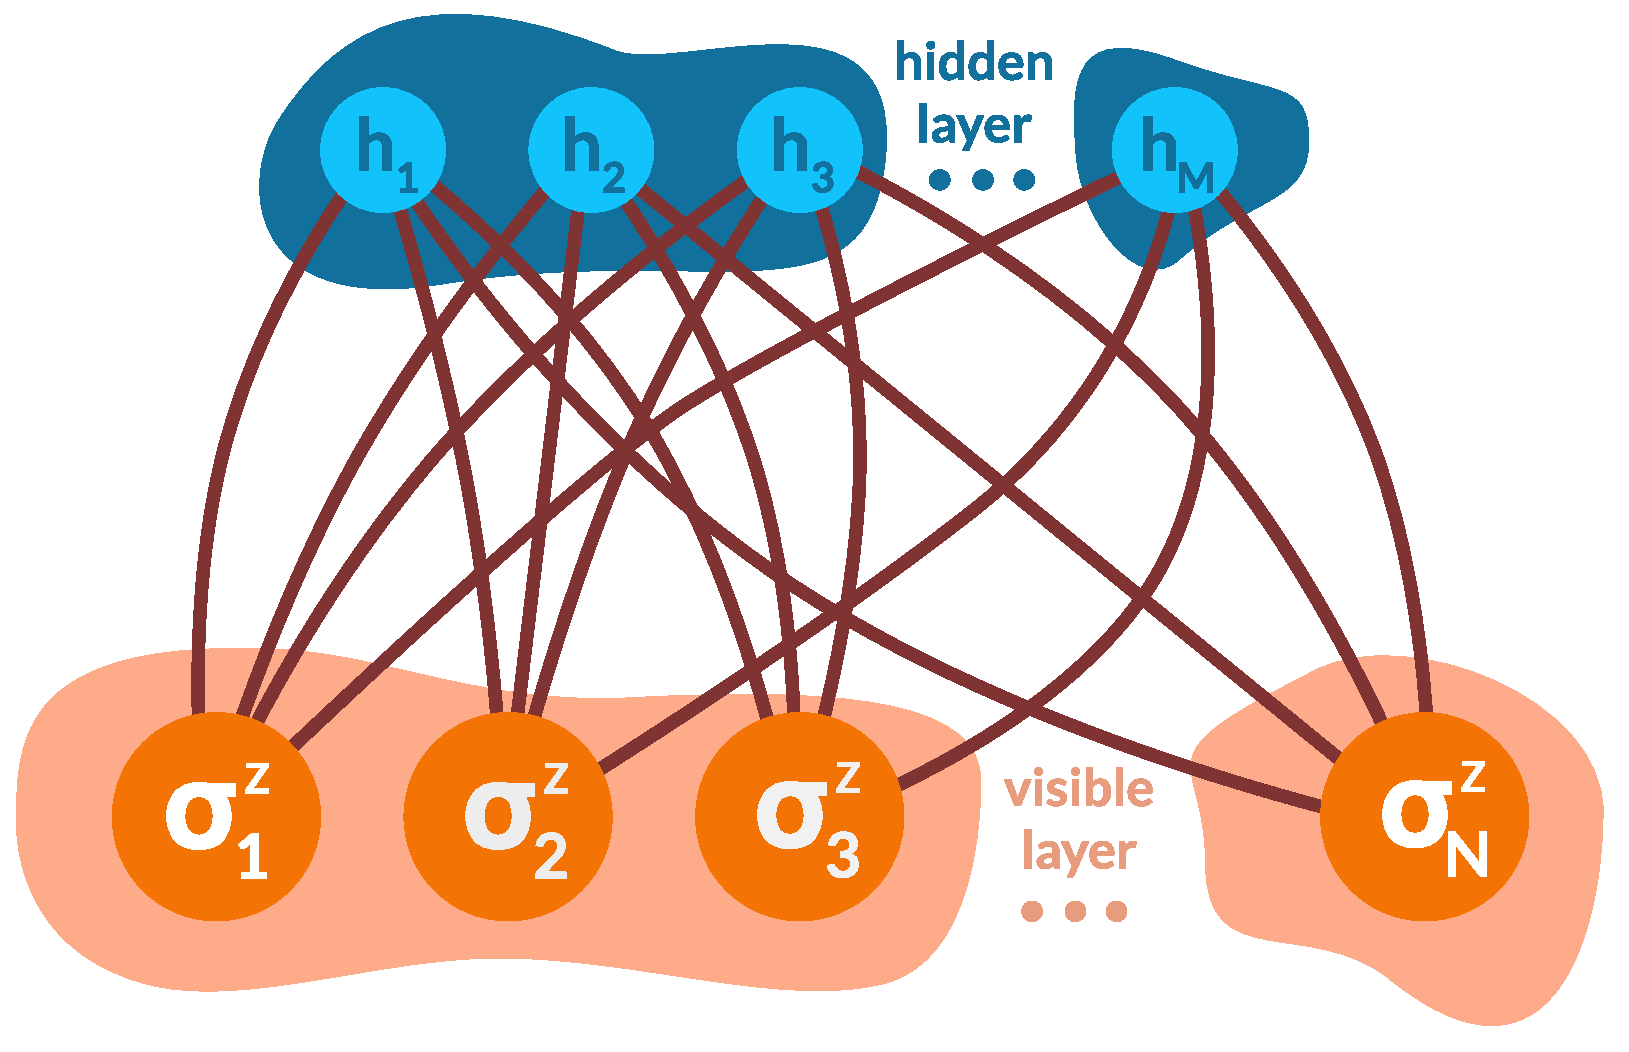
\includegraphics[width=0.5\textwidth]{figures/chapter3/rbm.pdf}
	\caption{Illustration of a restricted Boltzman machine (RBM) neural network.}
	\label{fig:rbm}
\end{figure}
\noindent
The qualification Restricted refers to the fact that the weights (interactions) only connect visible and hidden spins, and there are no weights amongst hidden spins. Because of this lack of inter-hidden layer connectivity of an RBM  all hidden variables can be traced out which leaves us with:
\begin{equation}
	\Psi(S,\mathcal{W}) = e^{\sum_i a_i s_i} \prod_{i=1}^{M} 2 \cosh(b_i + \sum_j W_{ij}s_j) \mathcomma
\end{equation}    
Following the algorithm from \cite{doi:10.1126/science.aag2302} we can train this network to efficiently represent the ground state of our Hamiltonian.


The reason we choose a NQS variational method is that one can readily compute the entanglement entropy in the (approximate) groundstate.
To exhibit dense entanglement at criticality in 2D systems, we wish to compute the entanglement entropy on a set of related theories that has tuneable set of degrees of freedom. A family of such theories are $Z_2\times Z_2 \ldots Z_2/Z_2$ multiple Ising matter fields gauged with $\mathbb{Z}_2$ symmetry on a 2+1D lattice \cite{Bukva:Registry}. These are extensions of the well known $Z_2/Z_2$ lattice gauge theory with Higgs fields from Fradkin and Shenker \cite{fradkinPhaseDiagramsLattice1979}. On the sites of a lattice, labeled by $\vec{r}$, we have $n$-Ising matter fields ($\sigma^i(\vec{r})$, $i=1\ldots n$) and on the links in the direction of the lattice vector $\hat{e}_\mu$ we have an Ising gauge field ($U(\vec{r},\hat{e}_{\mu})$. The action of a $d+1$ dimensional model on a hypercubic lattice is defined as:
	\begin{equation}
		\begin{split}
			&S(\sigma(\vec{r}), U(\vec{r},\hat{e}_{\mu})) =
			J \sum_{i=1}^n\sum_{\vec{r}, \mu} \sigma^i(\vec{r}) U(\vec{r},\hat{e}_{\mu}) \sigma^i(\vec{r} + \hat{e}_\mu)  \\ &+ K \sum_{\vec{r}, \mu \nu} 
			U(\vec{r},\hat{e}_{\mu}) U(\vec{r} + \hat{e}_\mu,\hat{e}_{\nu}) U(\vec{r}+\hat{e}_{\nu}+\hat{e}_{\mu},-\hat{e}_{\mu}) U(\vec{r}+\hat{e}_{\nu},-\hat{e}_{\nu}) \mathperiod
		\end{split}
	\end{equation}
	This action is invariant under the local $\mathbb{Z}_2$ gauge transformations:
	\begin{equation}
		\begin{split}
			\sigma^i(\vec{r}) &\rightarrow 
			= \sigma^i(\vec{r}) s(\vec{r}) \mathcomma \\
			U(\vec{r},\hat{e}_{\mu}) &\rightarrow s(\vec{r})U_\mu(\vec{r},\hat{e}_{\mu})s(\vec{r} + \hat{e}_\mu) \mathcomma
		\end{split}		
	\end{equation}
	where $s(\vec{r}) = \pm 1$. Though for $n=1$ there is famously no phase transition at $K=0$ as a function of $J$ illustrating the formal equivalence between the confining ($J<0$) and Higgs ($J>0$) phase of the $Z_2/Z_2$ theory, for any $n \geq 2$ there is a second order phase transition at finite $J$ between an disordered $J<0$ and ordered phase $J>0$ \cite{Bukva:Registry}. The phase transition belongs to the $p=2^{n-1}$-Potts universality class and is characterized by an expectation value of the (gauge invariant) registry order parameters $\langle \sigma^1\sigma^2\rangle$,  $\langle \sigma^1\sigma^3\rangle$, \ldots, $\langle \sigma^{n-1}\sigma^n\rangle$. We will use the product of all order parameters to measure all of them simulataneously $\langle \sigma_1^{n-1}\sigma_{2}^{n-1}\ldots \sigma_n^{n-1}\rangle =\prod_{i<j}\langle \sigma_i\sigma_j\rangle +\ldots $. This implies that the 2D quantum system corresponding to this system has a quantum phase transition with critical behavior at the corresponding point. The corresponding quantum Hamiltonian can be derived using transfer matrix formalism. Following \cite{transferMatrix1978,RevModPhys.51.659} we find a $Z_2$ gauged transverse field Ising Hamiltonian 
	\begin{align}
		\label{eq:gaugeHamiltonian} 
		H = &-\sum_{i, \vec{r}} \sigma_1^i(\vec{r}) - \sum_{\vec{r}, \mu} \tau_1(\vec{r},\hat{e}_{\mu})
		-\lambda \sum_i\sum_{\vec{r}, \mu} \sigma_3^i(\vec{r})\tau_3^\mu(\vec{r})\sigma_3^i(\vec{r}+\hat{e}_\mu) 
		\\ & 
		-\omega \sum_{\vec{r}, \mu \nu} \tau_3(\vec{r},\hat{e}_{\mu})\tau_3(\vec{r}+\hat{e}_\mu,\hat{e}_{\nu})\tau_3(\vec{r}+\hat{e}_\nu,\hat{e}_{\mu})\tau_3(\vec{r},\hat{e}_{\nu}) \mathcomma \nonumber
	\end{align}
	where now the matter fields $\sigma^i$ and the gauge field $\tau$ are Pauli matrices acting on sites and links of a 2D lattice, and we used that for a $Z_2$ symmetry the link is its own Hermitian conjugate $\tau(\vec{r}+\hat{e}_{\mu},-\hat{e}_{\mu})=\tau(\hat{r},\hat{e}_{\mu})$. The coupling coefficients $\lambda$ and $\omega$ can be related to $K$ and $J$ in the 2+1D classical action formulation, but the precise relation is unimportant. We shall set $\omega =0$ and keep $\lambda$ undetermined.  
	What is important for our NQS variational approach is that 
	physical states of this theory must satisfy the gauge invariance constraint. So therefore must the NQS itself. The local gauge transformations are generated by $G(\vec{r})=\prod_i\sigma_1^i(\vec{r})\prod_{\mu}\tau_1(\vec{r},\hat{e}_{\mu})$ at each site $\vec{r}$. Every physical state $\ket{\psi}$ must therefore obey
	\begin{equation}
		G(\vec{r}) \ket{\psi} = \ket{\psi}
	\end{equation}
	for every site $\vec{r}$ of the lattice. This constraint can easily be visualized in the $\tau_1$ and $\sigma_1$ basis Fig.\ref{fig:contraint}, basically every site needs to have $n+m =2 k, k\in\mathbb{Z}$ with $n$ the number of down spins on and $m$ the number of down-links emanating from the site. 
	
	\begin{figure}[H]
		\centering
		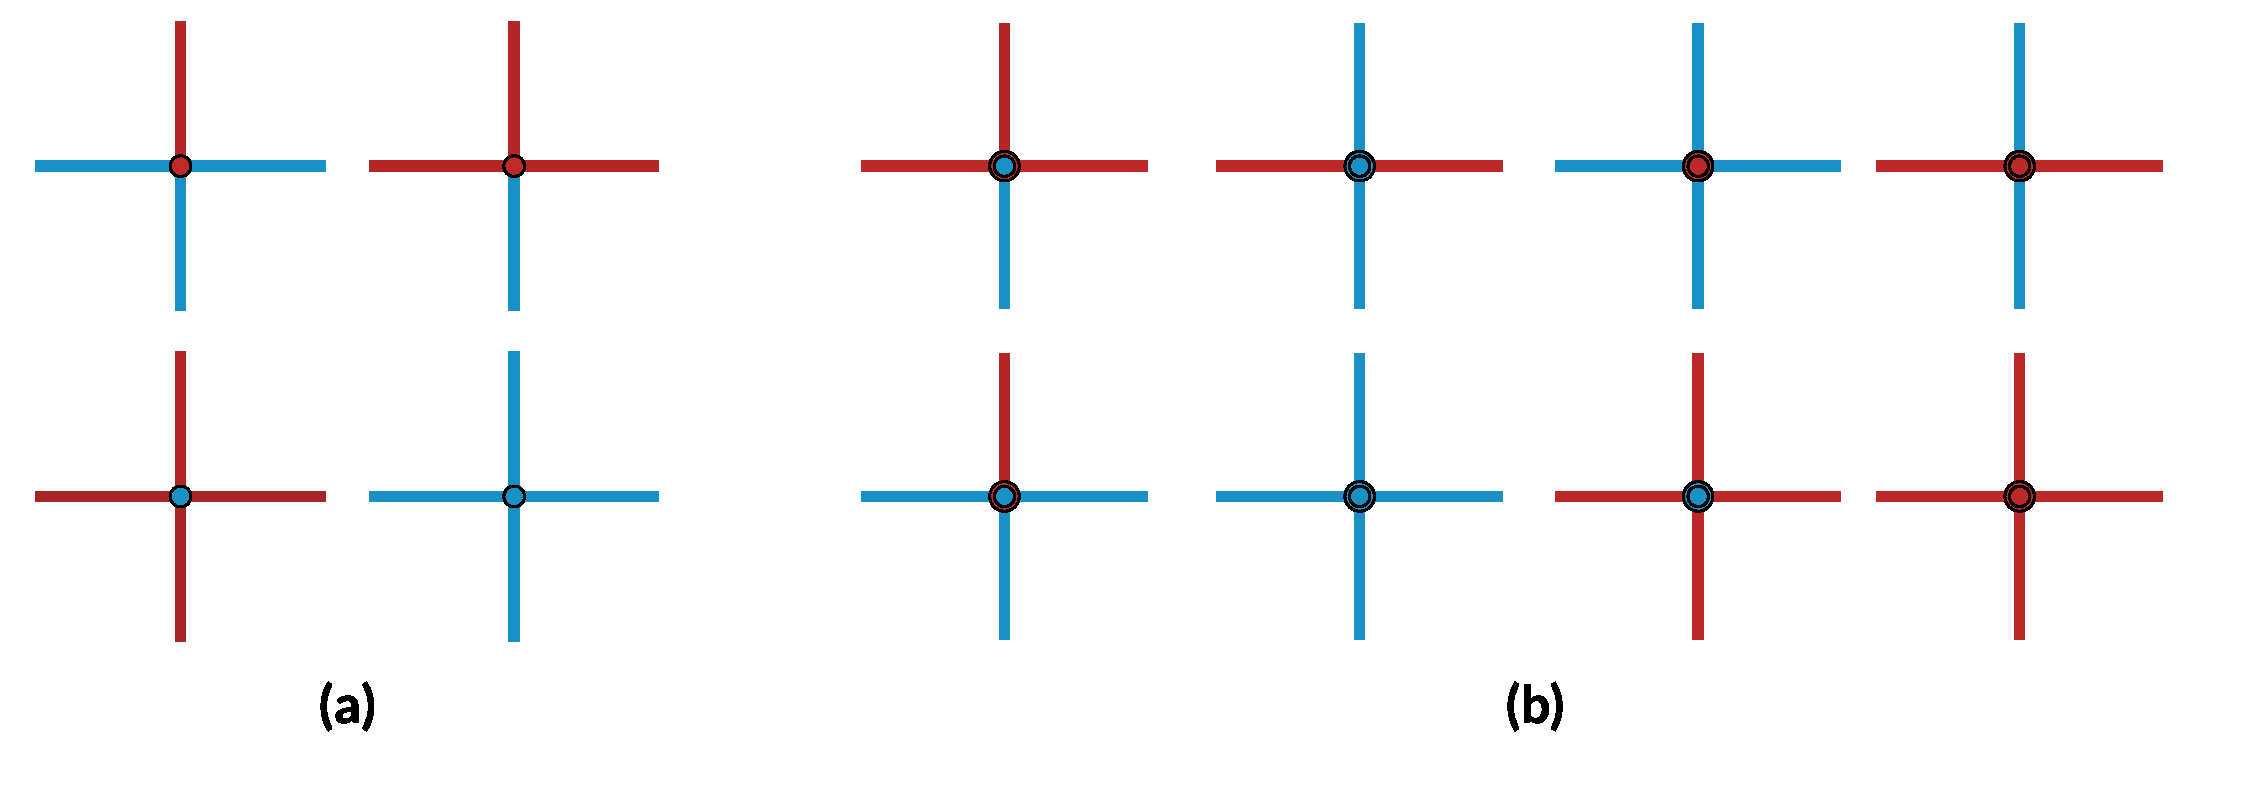
\includegraphics[width=0.65\textwidth]{figures/chapter3/constraint.pdf}
		\caption{Visualization of the gauge constraint in $\tau_1$ and $\sigma_1$ basis. \textcolor{myred}{Red} color represents down spins (-1) and \textcolor{myblue}{blue} up spins (+1). \textbf{(a)} Different gauge invariant combinations in the case of $Z_2 / Z_2$ theory. \textbf{(b)} Different gauge invariant configurations for the $Z_2 \cross Z_2 / Z_2$ theory. For the visual purposes spins at the nodes of a lattice for two fields are different sizes, so they can be distinguished in the diagram.}
		\label{fig:contraint}
	\end{figure}
	
	The NQS wavefunction itself is approximated by MCMC sampling. Due to the gauge constraint, this has to be done with care, because the naive Hilbert space is now larger than the space of physical states. We employ a simple updating procedure that always flips two matter spins, a matter spin and a link, or two links on a site to remain within the physical Hilbert space. For alternate approaches to NQS states for gauged lattice models, see \cite{luoGaugeEquivariantNeural2021}. 
	
	\section{Entanglement entropy}
	\label{sec:ee}
	
	The reason we resort to NQS to approximate the ground state is that entanglement or rather the entanglement entropy can be readily computed for such wavefunctions. Entanglement entropy is of course only a partial measure of entanglement, but to first approximation it should be able to quantify its denseness. Given a system described by a density matrix $\rho$ and divided into two parts, $A$ and $B$, then the entanglement entropy between these parts is defined as:
	\begin{equation}
		\label{eq:EE}
		S_A = -\tr \left[\rho_A \log \rho_A\right] ~,~~~~\rho_A =\text{Tr}_B\rho~.
	\end{equation}
	If the original state is pure, as is the case here, then $S_B=S_A$.\footnote{
		An important comment is that one has to be careful in computing the entanglement entropy in gauged theories, see e.g. \cite{Trivedi}. As our algorithm specifically only limits to physical states, this is not an issue, and we can use the standard expression Eq.(\eqref{eq:EE}).}
	
	Quite generally, for a system decomposable into two parts $A$ and $B$, the (ground)state can be written as
	\begin{equation}
		\ket{\Psi} = \sum_{i,j} c_{i,j} \ket{i}_A \otimes \ket{j}_B~.
		\label{eq:stateDecomp}
	\end{equation}
	The coefficients of the expansion $c_{i,j}$ can be combined in one probability-amplitude matrix where each element at the coordinates $i$,$j$ would be a probability-amplitude that we find the system with part $A$ being in the state $i$ and part $B$ being in the state $j$. 
	The entanglement entropy can be computed
	using Schmidt/Singular Value Decomposition (SVD); see \cite{Shi_2019} in the context of NQS or e.g. \cite{2011arXiv1109.0104M} in the contect of MCMC. We write the probability-amplitude matrix as:
	\begin{equation}
		c_{i,j} = U_{i,k}\Sigma_{k,l}V^\dagger_{l,j}~.
	\end{equation}
	If we label with $N_A$ and $N_B$ the sizes of parts $A$ and $B$ respectively, then $U, \Sigma$ and $V^\dagger$ are matrices of dimensions $N_A \cross N_A$, $N_A \cross N_B$ and $N_B \cross N_B$, where $\Sigma_{kl}=\sigma_k\delta_{kl}$ is a ``diagonal'' matrix with singular (i.e. non-negative real) values on the main diagonal and zeros otherwise. 
	Using this decomposition the entanglement entropy is easily seen to equal
	\begin{equation}
		S_A = -\sum_{i=0}^{\text{min}(N_A, N_B)} \sigma_i^2 \log \sigma_i^2 \mathperiod
	\end{equation}	
	In the variational NQS approach the wavefunction is represented probabilistically by an ensemble of $N_{\text{ens.}}$ states with $N_{\text{ens.}}=10^4$ as default choice. To compute the entanglement entropy from this subrepresentation, we follow \cite{Shi_2019}. These $N_{\text{ens.}}$ correspond to $N_{\text{conf}}\ll N_{\text{ens.}}$ different spin configurations, where the multiplicity $n_{\vec{s}}$ of each spin configuration is directly related to its weight $p_{\vec{s}}=n_{\vec{s}}/N_{\text{ens.}}$ in the ensemble. Algorithmically we can easily read off the non-vanishing spin configurations in subsystem $A$ and subsystem $B$, and construct the non-vanishing components of the matrix $c_{i,j}=\langle i,j|\psi_{\text{NQS}}\rangle$.	We hierarchically order the absolute value of the $|c_{i,j}|$. We make a reduced ansatz by only keeping the $N_{\text{red.}}$ largest values. This gives an $N_{\text{red.}}^{(A)}\times N_{\text{red.}}^{(B)} \geq N_{\text{red.}}$ matrix of $c_{i,j}^{\text{red.}}$.	In case one is interested in the entanglement entropy between exactly one half of the system and the other, then by symmetry $N_{\text{red.}}^{(A)}\times N_{\text{red.}}^{(B)} = N_{\text{red.}}$, and $N_{\text{red.}}$ should be chosen to be an exact square.	We then compute the entanglement entropy of $c_{i,j}^{\text{red.}}$ by Schmidt decomposition. 
	The accuracy of the entanglement entropy is controlled by the truncation $q=N_{\text{red.}}/N_{\text{ens}}$, and we can compare this to the accuracy in the groundstate energy when only sampled over the $N_{\text{red.}}$ most important contributors to the ensemble.
	
	There is one point one needs to pay special attention to.
	When computing the entanglement entropy for gauge theory in the above described way, it can happen that in constructing the matrix $c_{i,j}$ that the final state resulted from combining states $i$ and $j$ is not gauge invariant. In that case the probability of system reaching that state is zero. When creating matrix $c_{i,j}$ we need to check all elements and if the state they came from is not gauge invariant set those to zero. Doing this we ensure that only gauge invariant states contribute to the entanglement entropy. 
	
	
	\section{Dense entanglement at criticality or not?}
	
	The 2D lattice we choose will be square of size $N_{\text{lattice}}=3\times 3$ with periodic boundary conditions (PBC). We will consider the sequence of $(Z_2)^n/Z_2$ gauge theories that have $n=\{2,3,4\}$. 
	More than 4 matter fields or more lattice sites becomes computationally expensive. The NQS variational ansatz will have with $N_{\text{lattice}}$ visible and $M$ hidden nodes, with the ratio of two labeled as $\alpha = M/N$. We try four different configurations $\alpha =\{1,2,3,4\}$. The accuracy of the untruncated groundstate energy is expected to scale polynomially in $\alpha$ \cite{Evenbly2013}; $\Delta E_{\text{g.s}} = a\alpha^{-b}$. Unlike \cite{Evenbly2013}, the exact groundstate energy is not known for our models. However, studying the convergence of the NQS for $\alpha=1,2,3,4$ we can roughly see that increasing the number of hidden knows gives an improvement that decreases relatively to the number of hidden nodes, if we ignore the lowest result $\alpha=1$. This is represented in Fig.\ref{fig:DeltaE-gs}, where we
	have sampled over 50 different initial conditions, and estimated the accuracy of the groundstate by using bootstrap over those 50 initial configurations.
	
	\begin{figure}[H]
		\centering
		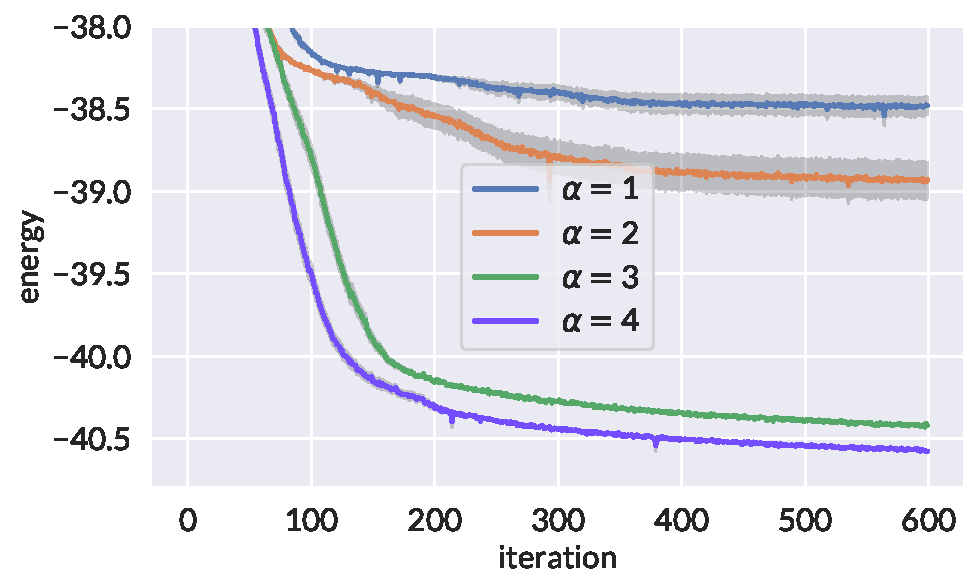
\includegraphics[width=0.7\textwidth]{figures/chapter3/energyvsepoch.pdf}
		\caption{The approach towards the optimal NQS ground-state wavefunction for the $Z^2/Z$ model measured through its energy as a function of learning epoch for $\alpha=1, 2, 3, 4$ for the value $\lambda=0.948, \omega=0$. Considering the $\alpha=1$ result an outlier, one sees an improved convergence as the number of hidden nodes $\alpha$ is increased. The average over 50 initial conditions is given as well as the standard error computed using bootstrap over 500 resamples.
		}
		\label{fig:DeltaE-gs}
	\end{figure}
	
	In this finite size system, there is no true instaneous phase transition, but its incipience is clearly visible in both the specific heat and the development of a finite order parameter for the registry symmetry. Fig.\ref{fig:regCv2fields} illustrates this. We clearly see the incipient second order phase transition as predicted for this model in \cite{Bukva:Registry}.
	\begin{figure}[t]
		\centering
		\mbox{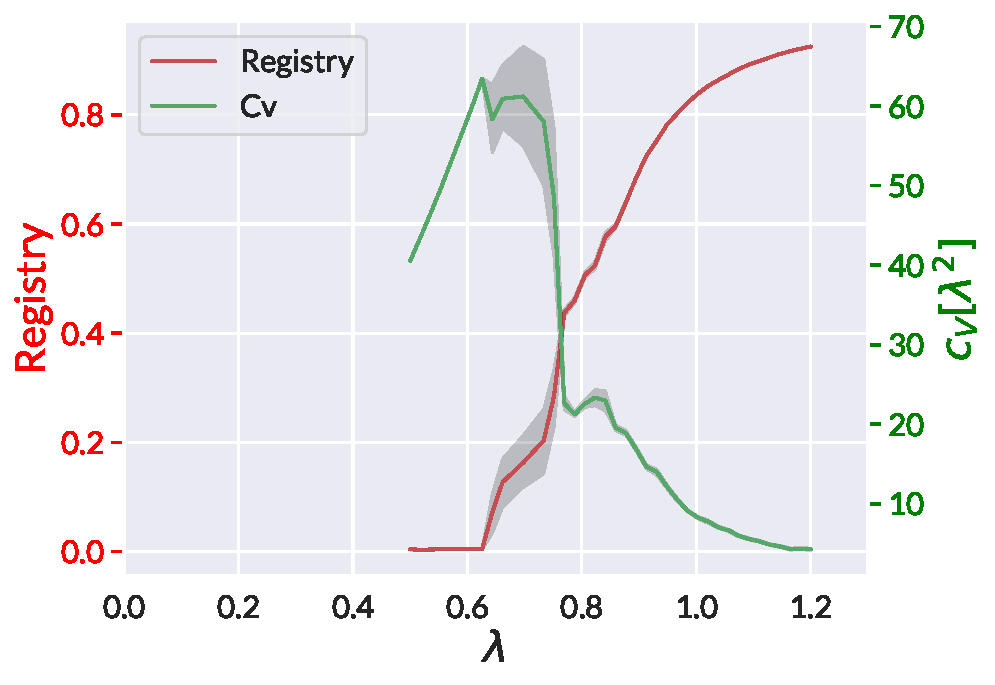
\includegraphics[width=0.33\textwidth]{figures/chapter3/2FieldsCVReg.pdf}
			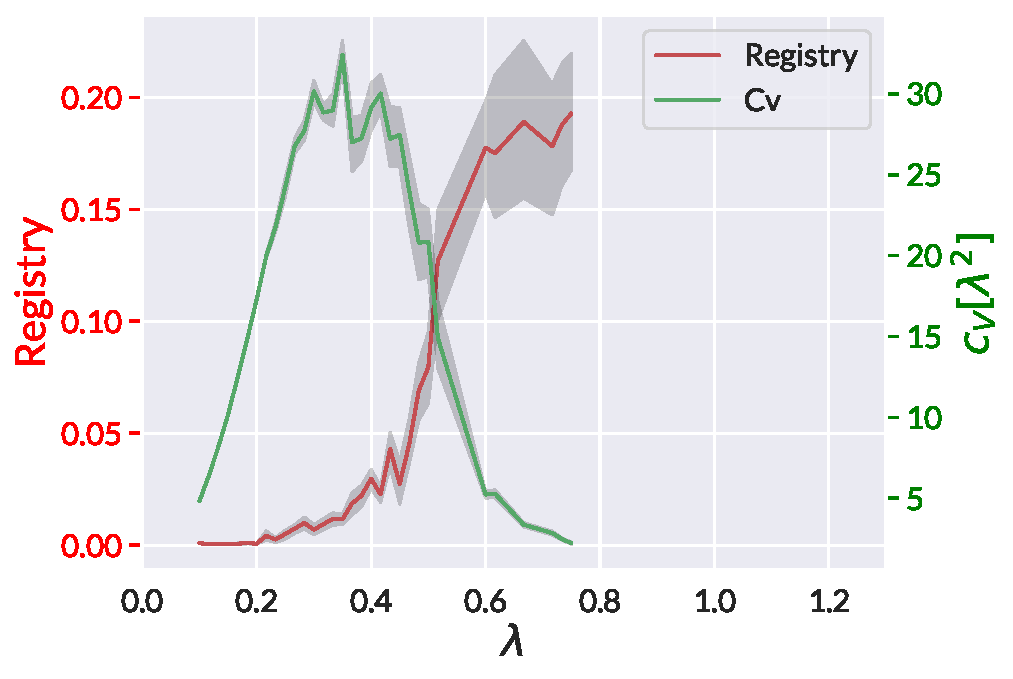
\includegraphics[width=0.33\textwidth]{figures/chapter3/3FieldsCVReg.pdf}
			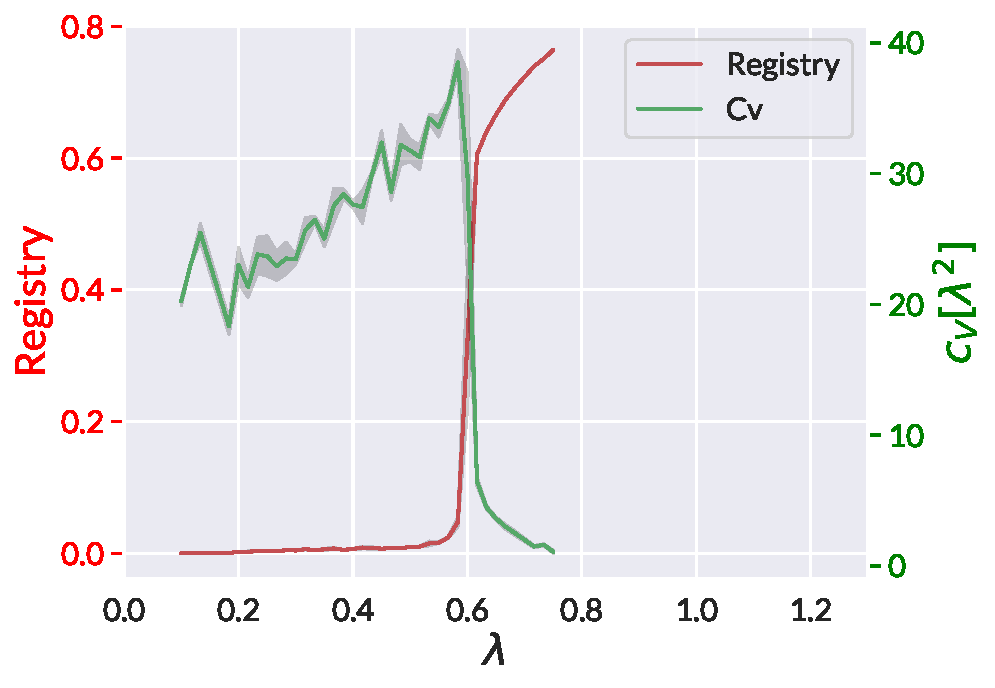
\includegraphics[width=0.33\textwidth]{figures/chapter3/4FieldsCVReg.pdf}}
		\caption{The specific heat $c_V=\frac{\partial \langle E\rangle_{NQS}}{\partial \lambda}$ (green) and registry order parameter $\langle{\cal O}_n\rangle =\langle\sigma_1^{n-1}\ldots\sigma_n^{n-1}\rangle_{NQS}$ (red) for the $Z_2^n/Z_2$ gauge theory for $n=2,3,4$ for $\omega=0$ as a function of $\lambda$ determined from the NQS wavefunction for $\alpha = 3$. The mean and standard deviation after are computed using bootstrap.  
		}
		\label{fig:regCv2fields}
	\end{figure}
	
	We can now test how entanglement also in  2D systems becomes denser {\em both} as we approach the critical point, {\em and} as we increase the number of degrees of freedom analogous to the central charge in 1D systems. Fig.\ref{fig:allEE} gives our results of the entanglement between $2/3$ and $1/3$ of the system. In the case of $3 \times 3$ system, dividing system exactly in half is not possible, the method we opted out for is the divisions along the secondary diagonal as in the Fig.\ref{fig:division}.
	\begin{figure}[t]
		\centering
		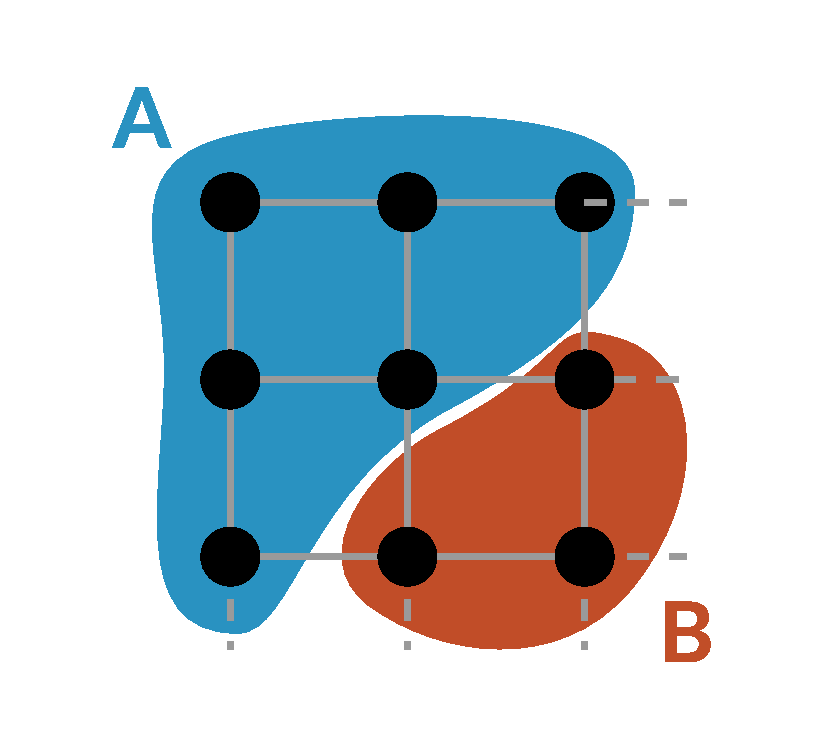
\includegraphics[width=0.35\textwidth]{figures/chapter3/latticeDivision.pdf}
		\caption{Illustration of the system division for a $3 \cross 3$ lattice used in our computations.}
		\label{fig:division}
	\end{figure}
	
	\begin{figure}[t]
		\centering
		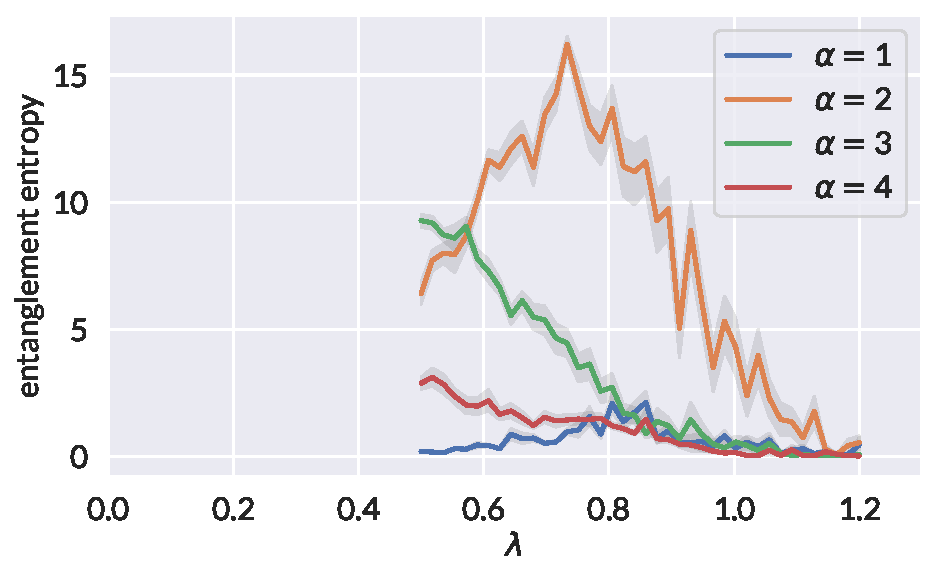
\includegraphics[width=0.33\textwidth]{figures/chapter3/EE_Ntwo.pdf}%
			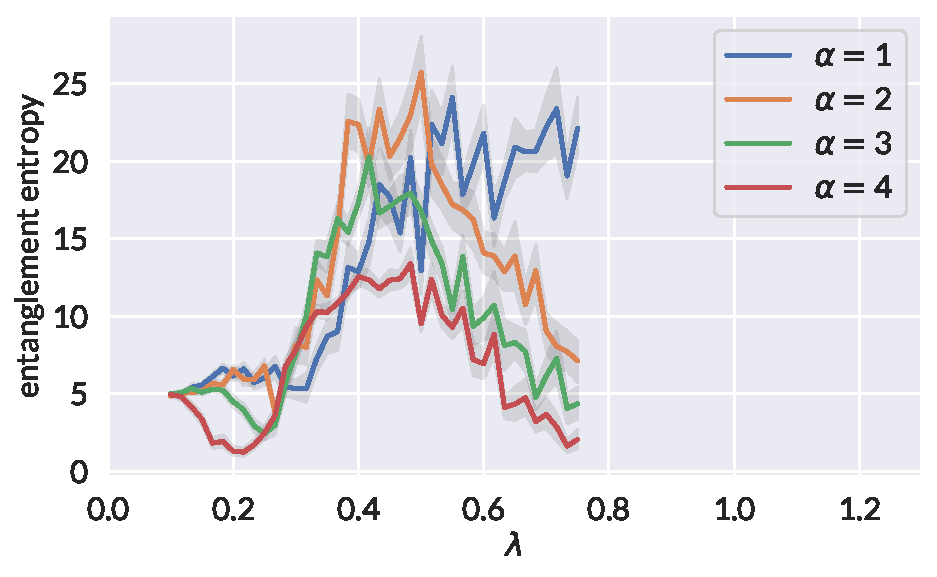
\includegraphics[width=0.33\textwidth]{figures/chapter3/EE_Nthree.pdf}%
			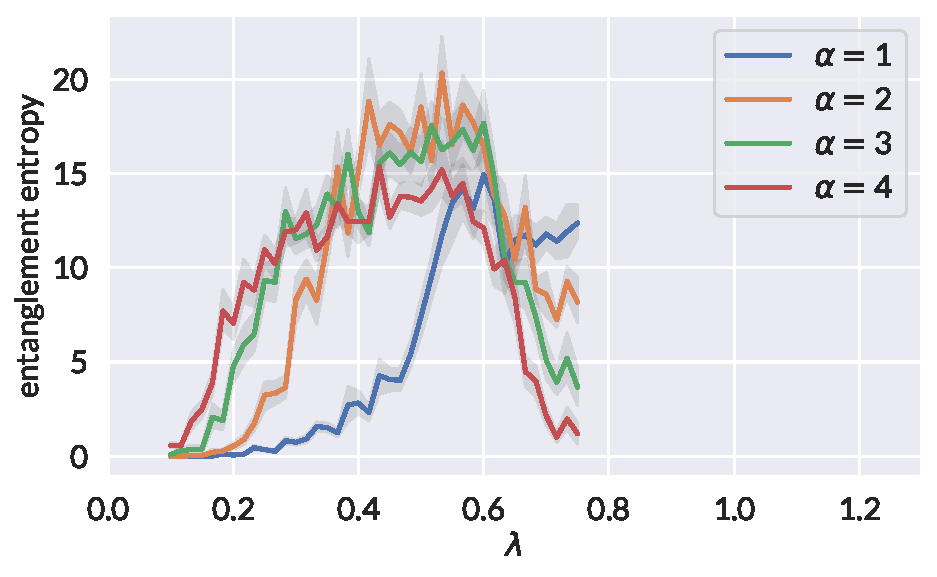
\includegraphics[width=0.33\textwidth]{figures/chapter3/EE_Nfour.pdf}\\
		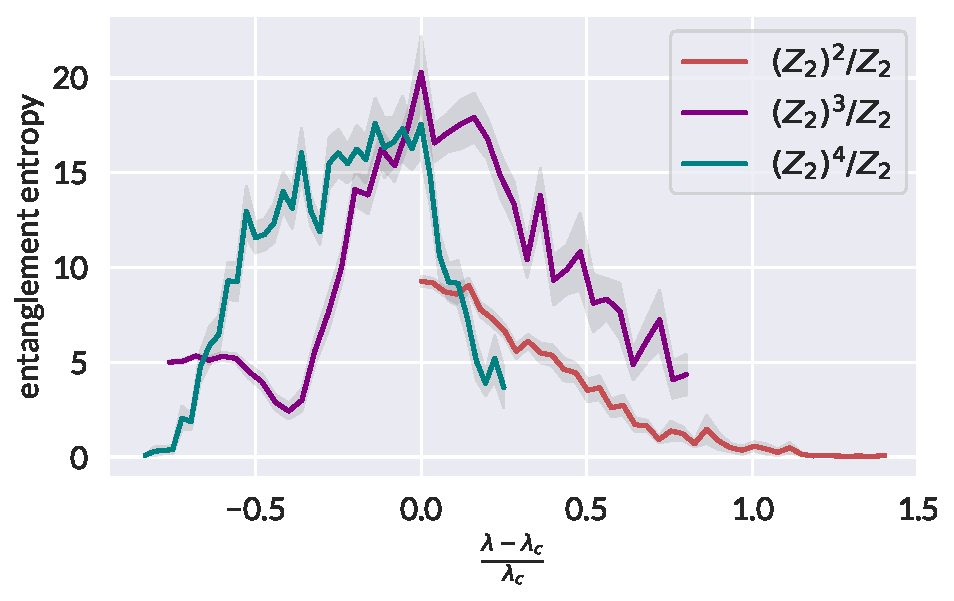
\includegraphics[width=0.33\textwidth]{figures/chapter3/EE_all_fieldsA3.pdf}%
			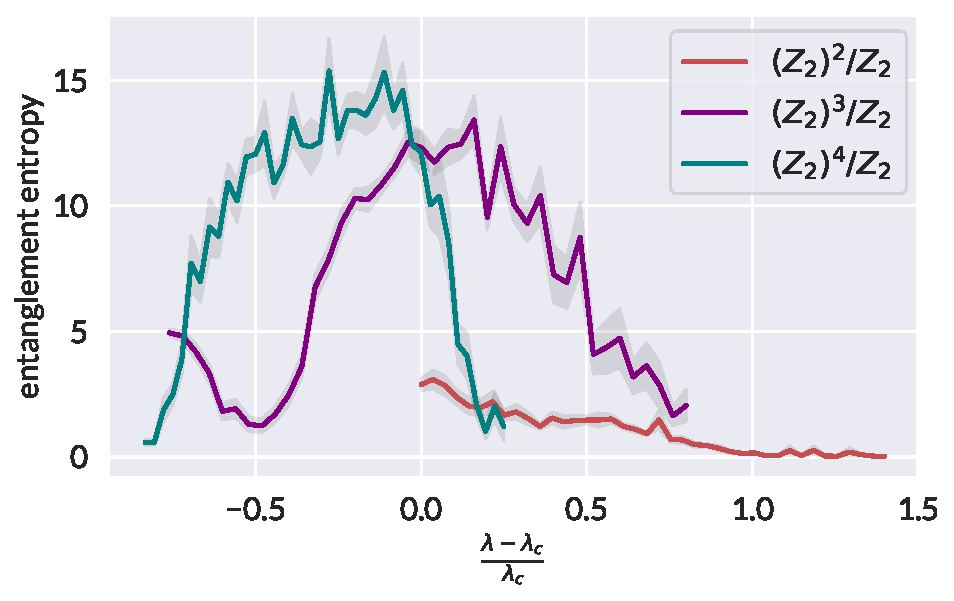
\includegraphics[width=0.33\textwidth]{figures/chapter3/EE_all_fieldsA4.pdf}\\
		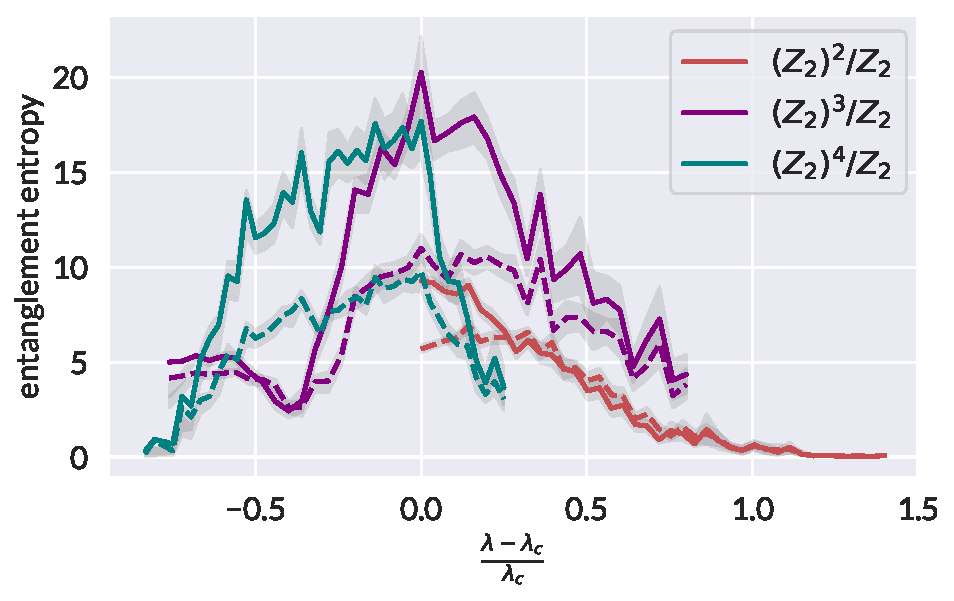
\includegraphics[width=0.33\textwidth]{figures/chapter3/EE_alpha_four_diffNsamples.pdf}
		\caption{The entanglement entropy $S_{2/3}$ of $2/3$ of the $3 \times 3$ system entangled with the other 1/3 for the $N_{\text{red.}}=10^4$ truncated (see text) NQS groundstate of $Z_2^n/Z_2$ gauge theories averaged over 50 initial conditions. The top row shows the dependence on the number of hidden variables as a function of $\lambda$ for $N_{\text{red.}}=10^4$: 
			Left is the result for $n=2$ for $\alpha=1,2,3,4$; middle for $n=3$; right for $n=4$. This estimates the error in the entanglement entropy. The middle
			row shows the dependence on $n$ rescaled to $\lambda_{\text{red.}} =\frac{\lambda-\lambda_c}{\lambda_c}$; left for $\alpha=3$, right for $\alpha=4$ for $N_{\text{red.}}=10^4$. No discernible increase in the entanglement entropy as a function of $n$ is seen. The bottom row shows the dependence on $N_{\text{red.}}=10^4$ (solid line) and $N_{\text{red.}}=10^3$ (dashed line).}
		\label{fig:allEE}
	\end{figure}
	Fig.\ref{fig:allEE} and specifically the middle row of Fig.\ref{fig:allEE} shows the results of the entanglement entropy for the sequence of $Z_2^n/Z_2$ theories as a function of the relative coupling $\lambda-\lambda_c/\lambda_c$ w.r.t. the criticial point.
	Initially the entanglement entropy does increase when going from 2 to 3 fields, but then stays the same when we added another 4th field. Though the numerical results are not super smooth, and there is a slight increase for $\alpha=4$, we expect a linear increase and this is clearly not there. There are several possible explanations for this. One is that finite size effects due to computational limitations do have a direct impact. This cannot be ruled out, but the fact that the entanglement entropy does not change much with the increase in $\alpha$ suggests otherwise. Already $\alpha=1$ appears sufficient to represent all the entanglement in the system. Another possible explanation for the relation between entanglement entropy and the number of matter fields is that increasing number of fields would require an increase in the $N_{\text{red.}}$. From the right figure in the bottom row of Fig.\ref{fig:allEE} we see that increase of $N_{\text{red.}}$ lead to the increase in the entanglement entropy. We are again computationally limited here as a further increase in the number of required states would cause memory issues. 	
	
	\section{Discussion}
	\label{sec:conclusion}
	Having presented our results, we must leave a verification whether entanglement entropy scales with the number of degrees of freedom also at a 2D critical point an open question. Surprisingly, within the limitations of our numerics in the $Z_2^n/Z_2$ sequence of models we studied this appears not to be the case. We cannot fully rule out that a technical/computational limitation is the cause, but we have performed extensive tests and the code faithfully reproduces the known 1D results (see Appendix). One possibility to overcome computational limitations is to move away from the traditional Monte Carlo sampling and using more direct approach like equivariant flow-based sampling \cite{Kanwar_2020} or generative models \cite{medvidovic2021generative}. We leave this for future research.
	
	\section*{Acknowledgments}

	We are especially grateful to Giuseppe Carleo and Matija Medvidovi\' c for their help in setting up NQS for gauged models.
	We thank Jan Zaanen for discussions and his insistence that this should be tested in models with $d>1$.
	This research was supported 
	in part by the Dutch Research Council
	(NWO) project 680-91-116 ({\em Planckian Dissipation and Quantum Thermalisation: From
		Black Hole Answers to Strange Metal Questions.}) and
	by the Dutch Research
	Council (NWO)/Ministry of Education.
	
	\section{Appendix}
	\subsection{NQS States and Entanglement for 1D transverse field Ising Model}
	Given that we have such an unexpected and curious result, it behooves an in depth exhibition of the validity of our approach.
	Here we compute the known entanglement entropy in a 1D transverse Ising model using exactly the same algorithm.
	These results agree with the theoretical expectation as well as the numerical NQS results of \cite{Shi_2019}.
	We have parametrized the 1D transverse field Ising model Hamiltonian analogous to Eq.(\eqref{eq:gaugeHamiltonian})
	\begin{align}
		H_{\text{TI-1D}} = &-\sum_{\vec{r}} \sigma_1(\vec{r})
		-\lambda \sum_{\vec{r}, \mu} \sigma_3(\vec{r})\sigma_3(\vec{r}+\hat{e}_\mu)
	\end{align}
	and use a $N=16$ site system
	with periodic boundary conditions.
	The results are on Fig.\ref{fig:TI-1D}. One sees the increase in entanglement as one approaches the critical value $\lambda_c=XX$ consistent with the notion of dense entanglement. 
	\begin{figure}[H]
		\centering
		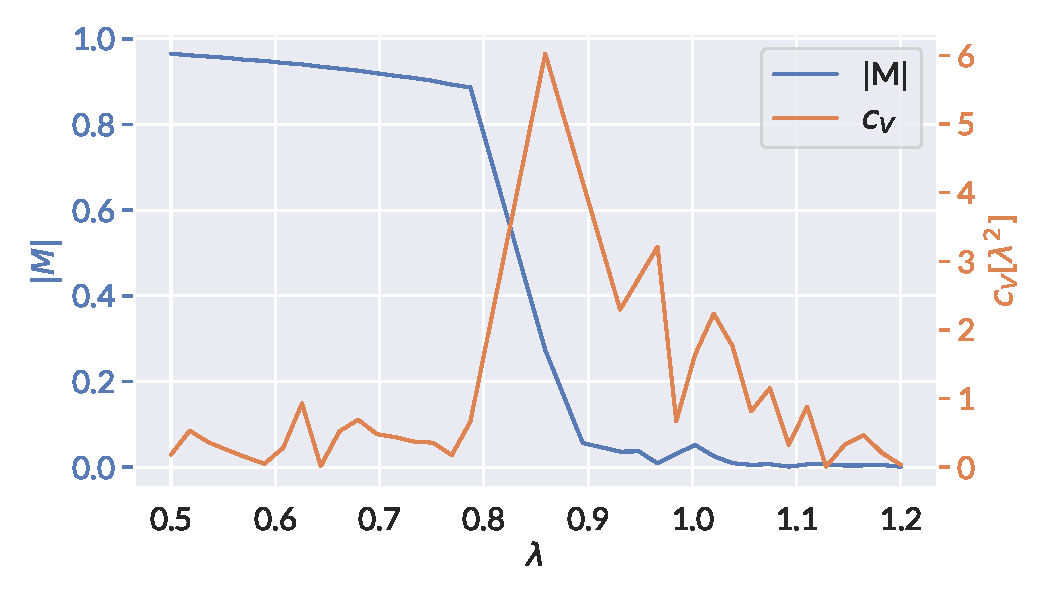
\includegraphics[width=0.4\textwidth]{figures/chapter3/IsingMagCv.pdf}
		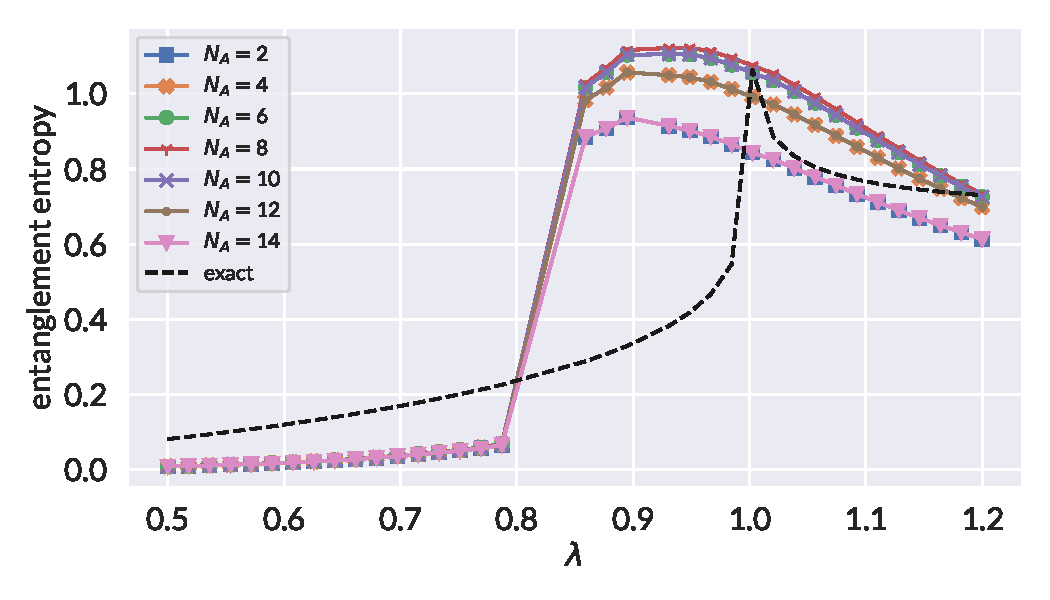
\includegraphics[width=0.4\textwidth]{figures/chapter3/IsingEE.pdf}
		\caption{Left: The specific heat and $Z_2$ order parameter of the 1D Ising model as a function of $\lambda$.
			Right: The entanglement entropy both as a function of $\lambda$ and as a function of boundary site $s=2,4,6,8,10,12,14$ between subsystem $A$ and subsystem $B$ (the boundary site is the last site that is included in $A$.). The dashed line is the CFT result in the continuum limit.}
		\label{fig:TI-1D}
	\end{figure}